% https://github.com/tribler/Tribler/wiki
% https://github.com/Tribler/tribler/wiki/Anonymous-Downloading-and-Streaming-specifications
% Screenshots voor tribler anonymous tunnels

\section{Tribler}
	\label{scc:tribler}
	In this section an overview of Tribler and its components is presented. We describe the new version that uses anonymous tunnels in depth. Furthermore, we look at what specific dependencies Tribler relies on.

	Tribler is a fully decentralized peer-to-peer file sharing system developed by the Parallel and Distributed Systems group at Delft University of Technology. It has been in development for over nine years and has a very mature and well-established code base. It allows users to search for and share files in a fully decentralized way. This decentralized nature of Tribler has several advantages over existing file sharing systems. The lack of a centralized component makes it very scalable and practically impossible to bring down.

	An experimental version of Tribler is currently available that includes a Python implementation of a Tor-like protocol. This enables users to share files anonymously and securely. By encrypting and routing traffic over a circuit of nodes, it ensures the communicating parties are oblivious of each other's virtual and physical location.
	
	\subsection{Downloading files}
		Tribler uses the torrent protocol\footnote{http://www.bittorrent.org/beps/bep\_0003.html} for downloading files.Torrent files contain metadata about the files that will be downloaded. The torrent protocol is peer-to-peer and this means that an user downloads from multiple seeders. Information about possible seeders is maintained by a tracker that can be queried about the available seeders. Tribler is using the libtorrent library as implementation of the torrent protocol. This library is licensed as open source software and we are allowed to use or modify it.
		
		Torrent files can be found using the graphical user interface (GUI) of Tribler. Users enters their search query in a search bar and Tribler will return the results matching the search criteria. A family filter has been added to Tribler to filter out adult content. The underlying search is done using Dispersy which will be described in Section \ref{sec:dispersy}.
	
	\subsection{Anonymous tunnels}
		\label{sec:anonymoustunnels}
			Recently, the research team of Tribler started to work on the implementation of anonymous downloads. Pull request\footnote{http://oss-watch.ac.uk/resources/pullrequest} 525 on the Tribler Github page \cite{pullrequest525} is an experimental build of Tribler with the implementation of anonymous communications. The anonymous communication is achieved by using a Tor-like protocol. This protocol has been implemented in Python and uses a three-hop circuit for anonymous communication. Three-hop means that data travels over three nodes before it reaches the destination, to add anonymity. Note that Tribler does not use the Tor network, only a Tor-like protocol with UDP connections.
			
			The anonymous tunnels are implemented in the Python module \emph{Tribler.community.anontunnel}. Taking the code as reference, we now describe various details of the anonymous tunnels.
			
			\begin{itemize} 
				\item The circuit setup is using the Diffie-Hellman key exchange protocol to establish a secure connection. The M2Crypto library which is explained in Subsection \ref{sec:m2crypto}, is used for the Diffie-Hellman protocol.
				\item The experimental code is using the Socks5\footnote{http://www.ietf.org/rfc/rfc1928.txt} protocol for communication with other nodes (see figure \ref{fig:onion_encryption_decryption_socks5}). This code has been written by the Tribler team.
				\item Dispersy is used as synchronization system. 
				\item A circuit can be in four states: ready, extending, to be extended or broken.
				\item There are nine different messages that can be send amongst nodes.
			\end{itemize}
			
			In order to test the anonymous connections and the download speed, a special anonymous tab has been built into Tribler. Clicking on this tab brings up a graph of the current anonymous network as a graph. It also logs the circuit events such as the extend or creation of a circuit. When enough anonymous proxies are online, a 50 MB test download file should start to download.
			
			\begin{figure*}[!htb]
				\centering
				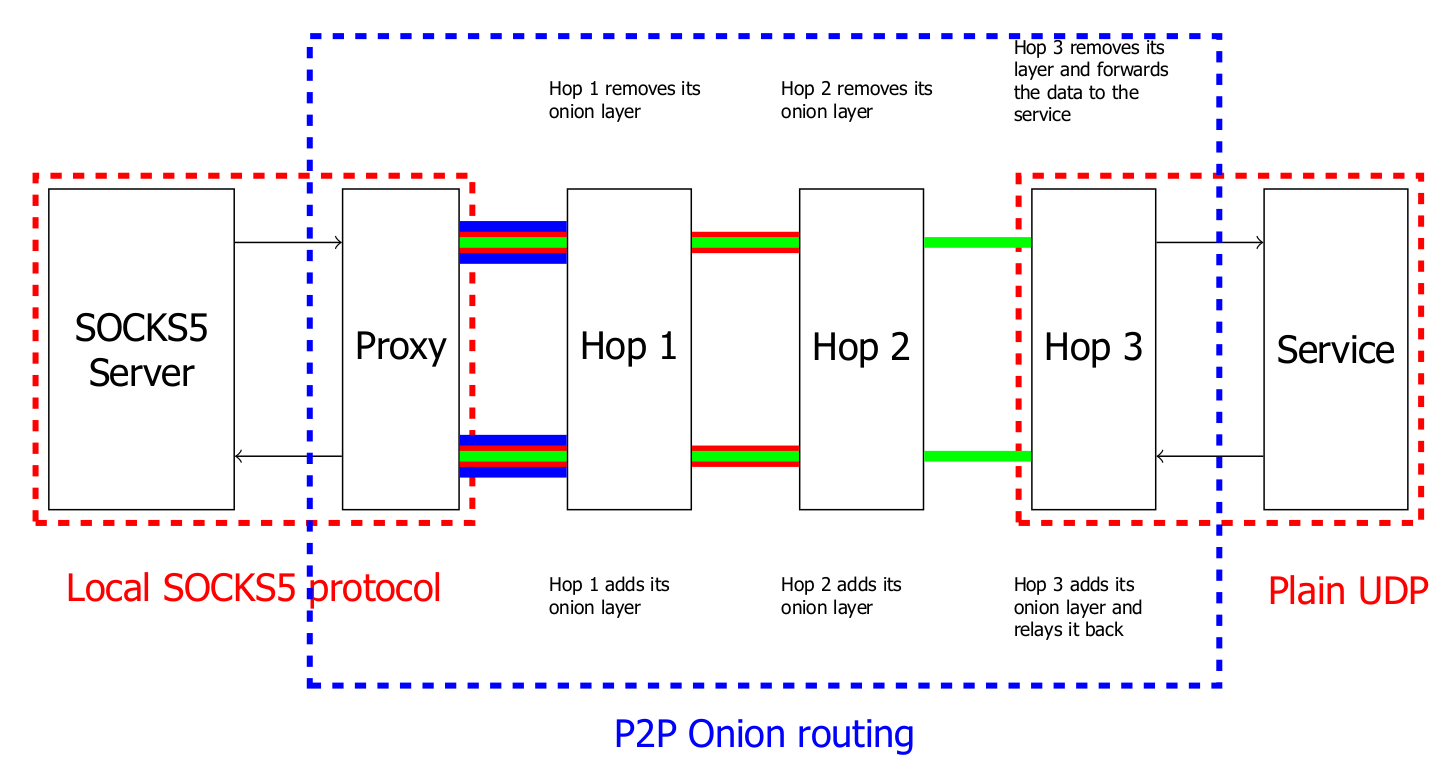
\includegraphics[width=\textwidth]{graphics/onion_encryption_decryption_socks5.png}
				\caption{The onion encryption and decryption used by the anontunnels. Taken from https://github.com/Tribler/tribler/wiki/Anonymous-Downloading-and-Streaming-specifications}
				\label{fig:onion_encryption_decryption_socks5}
			\end{figure*}

	\subsection{Security}
		Tribler makes use of cryptographic functions to encrypt data and make secure communication possible. Security is a big issue in the world of peer-to-peer networks. Not only do we want anonymous downloads, we also want confidentiality and integrity of our data. Confidentiality means that unauthorized parties cannot see the exact content of the information. This could be achieved by encrypting the data. Integrity of the data means that the data is protected from being modified by other parties. Confidentiality and integrity are important when communicating. When we are sending confidential data over the internet, it would not be beneficial if everyone has access to the message and can read what is being send. Integrity can play a role when transferring money to another bank account: we do not want an adversary to temper with the amount of money that is being transferred.
		
		Some popular open source frameworks exists for these cryptographic tasks. A popular project is OpenSSL \cite{openssl}. OpenSSL implements the popular SSL and TLS protocols\footnote{http://tools.ietf.org/html/rfc5246}. These are cryptographic protocols that provides security when communicating over the internet. Besides that, OpenSSL provides libraries for various encryption and decryption protocols such as 3DES\footnote{http://tools.ietf.org/html/rfc2420}, RSA \footnote{http://www.ietf.org/rfc/rfc2437.txt} and RC4 \footnote{http://tools.ietf.org/html/rfc4757}. OpenSSL also supports key exchange protocols such as Diffie-Hellman\footnote{http://www.ietf.org/rfc/rfc2631.txt}.
		
		OpenSSL is written in the C programming language. To use the OpenSSL libraries in Python, one could use pyopenssl \cite{pyopensslgithub}, a interface for OpenSSL or M2Crypto \cite{m2cryptogithub} (M2Crypto stands for 'Me Too Crypto'), an OpenSSL wrapper. Tribler makes use of the M2Crypto library. The M2Crypto library provides many implementations of popular cryptographic protocols that are used for secure communication.
		
	\subsection{Dispersy}
	\label{sec:dispersy}
		Tribler makes use of Dispersy. As elaborated by Zeilemaker et al; Dispersy \cite{zeilemaker2013dispersy} is a fully decentralized system for data bundle synchronization. This means that data is exchanged between peers to make sure they are up-to-date with the same information. The system is designed in such a way that it is capable of running in a challenging network environment. Such an environment is often characterized by:
		\begin{itemize}
			\item Nodes randomly joining and leaving.
			\item Delays in the network.
			\item Nodes having different networking speeds (Edge, 3G, WiFi).
			\item Nodes often being behind routers with Network Address Translating (NAT) firewalls.
		\end{itemize}
		
		All communication done by Dispersy uses UDP. Because up to 64\% of the Internet is behind a NAT, they can use UDP NAT-firewall puncturing mechanisms\cite{zeilemaker2013dispersy}.
		
		In Dispersy, each node has a candidate list. A candidate list is a list of active connections within the node's overlay. A Dispersy node synchronizes in five steps:
		
		\begin{enumerate}
			\item First it selects a node from its candidate list.
			\item It then selects a range of bundles to synchronize.
			\item The node creates a Bloomfilter \footnote{"A Bloom filter is a space-efficient probabilistic data structure, conceived by Burton Howard Bloom in 1970, that is used to test whether an element is a member of a set.", quoted from http://en.wikipedia.org/wiki/Bloom\_filter} by hashing the selected bundles.
			\item Then the node sends the created Bloomfilter to the selected node.
			\item Finally, it pauses for a fixed interval to go back to step 1.
		\end{enumerate}
		
		The candidate list is divided into three sections: trusted nodes, nodes that have been successfully contacted in the past and nodes that have been connected in the past either trough an introduction-request or nodes that have been introduced.
		
		A Bloomfilter uses a hash area consisting of \emph{N} bits, initially all set to zero. For each item that needs to be stored in the Bloomfilter, \emph{K} distinct addresses are generated using a hash of the item. The bits addressed in the Bloomfilter are then set to one. To check if an item is part of a Bloomfilter, one only has to generate the hash of that item and check if the addresses that are generated by the hash are one in the Bloomfilter.
		
		After benchmarking Dispersy against Cassandra\cite{zeilemaker2013dispersy} (the database system used by Facebook), Zeilemaker et al. came to the conclusion that Dispersy performs better than Cassandra. By using Bloomfilters, Dispersy can scale to over 100,000 bundles to synchronize.
	
		\begin{figure*}[!t]
			\centering
			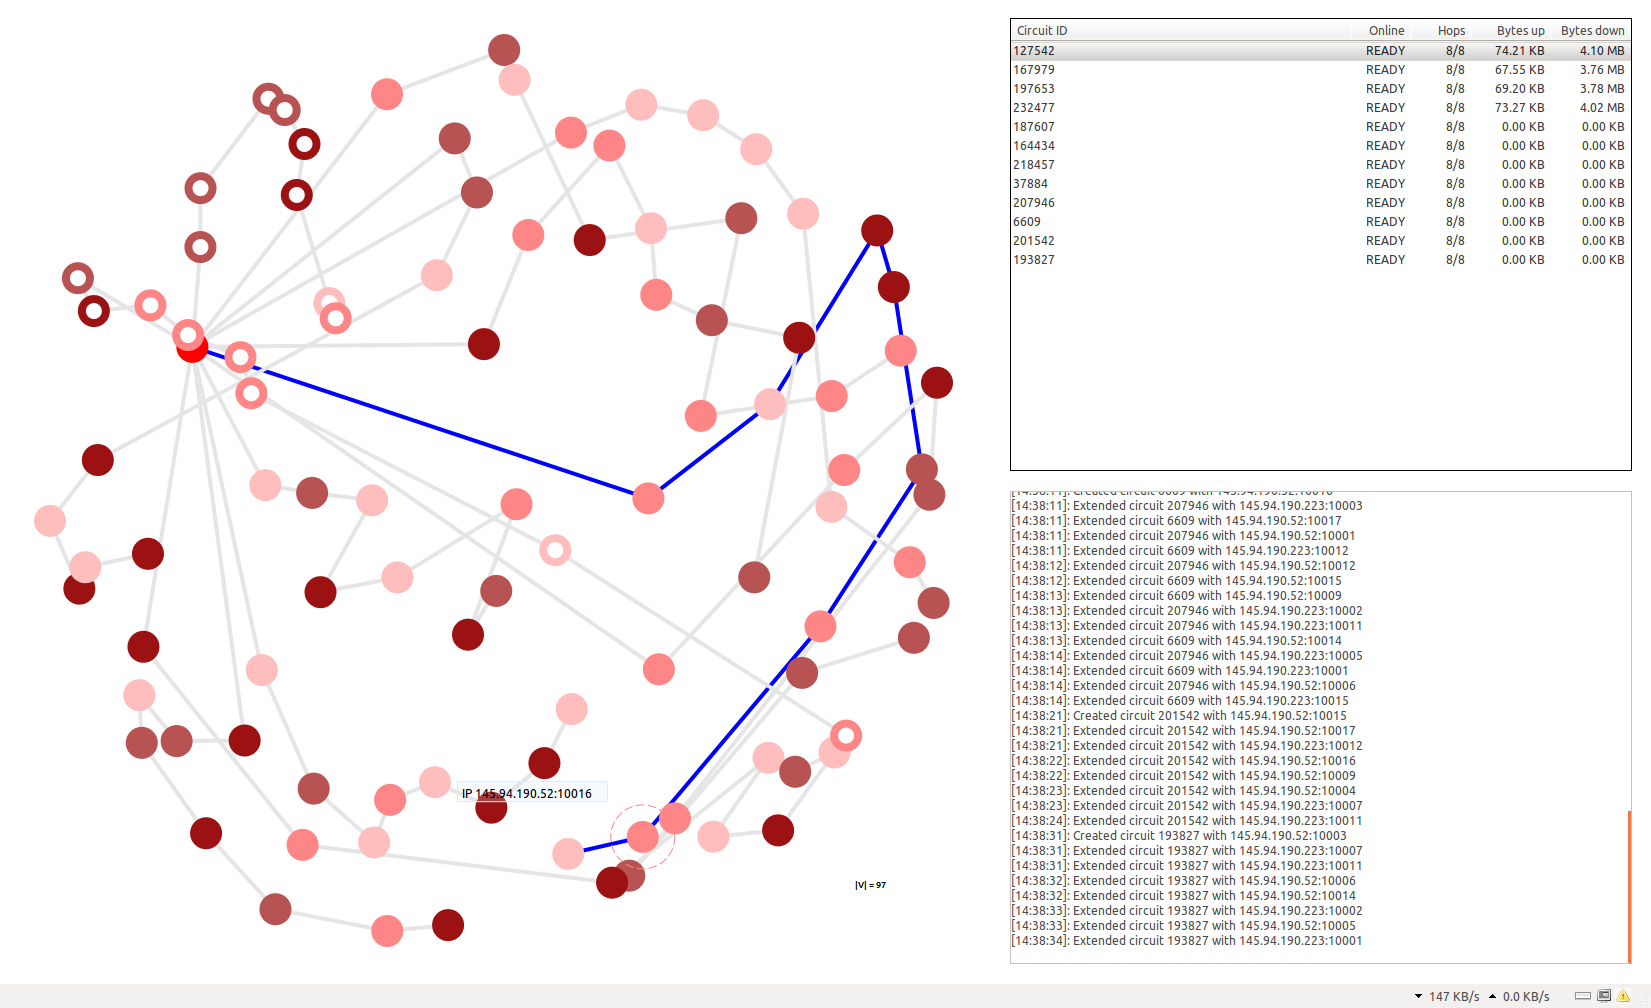
\includegraphics[width=0.8\textwidth]{prior-work/8hop.png}
			\caption{The graphical user interface in Tribler that shows the anonymous network.}
			\label{fig:anon_downloads}
		\end{figure*}